%%
%% This is file `sample-acmlarge.tex',
%% generated with the docstrip utility.
%%
%% The original source files were:
%%
%% samples.dtx  (with options: `acmlarge')
%% 
%% IMPORTANT NOTICE:
%% 
%% For the copyright see the source file.
%% 
%% Any modified versions of this file must be renamed
%% with new filenames distinct from sample-acmlarge.tex.
%% 
%% For distribution of the original source see the terms
%% for copying and modification in the file samples.dtx.
%% 
%% This generated file may be distributed as long as the
%% original source files, as listed above, are part of the
%% same distribution. (The sources need not necessarily be
%% in the same archive or directory.)
%%
%%
%% Commands for TeXCount
%TC:macro \cite [option:text,text]
%TC:macro \citep [option:text,text]
%TC:macro \citet [option:text,text]
%TC:envir table 0 1
%TC:envir table* 0 1
%TC:envir tabular [ignore] word
%TC:envir displaymath 0 word
%TC:envir math 0 word
%TC:envir comment 0 0
%%
%%
%% The first command in your LaTeX source must be the \documentclass
%% command.
%%
%% For submission and review of your manuscript please change the
%% command to \documentclass[manuscript, screen, review]{acmart}.
%%
%% When submitting camera ready or to TAPS, please change the command
%% to \documentclass[sigconf]{acmart} or whichever template is required
%% for your publication.
%%
%%
\documentclass[acmlarge]{acmart}
\usepackage{lipsum}
%\usepackage{amsmath}
%\usepackage{amssymb}
%\usepackage{graphicx}
\usepackage[linesnumbered]{algorithm2e}

\usepackage{listings}% http://ctan.org/pkg/listings
\lstset{
  basicstyle=\ttfamily,
  mathescape
}

%%
%% \BibTeX command to typeset BibTeX logo in the docs
\AtBeginDocument{%
  \providecommand\BibTeX{{%
    Bib\TeX}}}

%% Rights management information.  This information is sent to you
%% when you complete the rights form.  These commands have SAMPLE
%% values in them; it is your responsibility as an author to replace
%% the commands and values with those provided to you when you
%% complete the rights form.
\setcopyright{acmcopyright}
\copyrightyear{2022}
\acmYear{2022}
\acmDOI{XXXXXXX.XXXXXXX}


%%
%% These commands are for a JOURNAL article.
\acmJournal{POMACS}
\acmVolume{37}
\acmNumber{4}
\acmArticle{111}
\acmMonth{8}

%%
%% Submission ID.
%% Use this when submitting an article to a sponsored event. You'll
%% receive a unique submission ID from the organizers
%% of the event, and this ID should be used as the parameter to this command.
%%\acmSubmissionID{123-A56-BU3}

%%
%% For managing citations, it is recommended to use bibliography
%% files in BibTeX format.
%%
%% You can then either use BibTeX with the ACM-Reference-Format style,
%% or BibLaTeX with the acmnumeric or acmauthoryear sytles, that include
%% support for advanced citation of software artefact from the
%% biblatex-software package, also separately available on CTAN.
%%
%% Look at the sample-*-biblatex.tex files for templates showcasing
%% the biblatex styles.
%%

%%
%% The majority of ACM publications use numbered citations and
%% references.  The command \citestyle{authoryear} switches to the
%% "author year" style.
%%
%% If you are preparing content for an event
%% sponsored by ACM SIGGRAPH, you must use the "author year" style of
%% citations and references.
%% Uncommenting
%% the next command will enable that style.
%%\citestyle{acmauthoryear}


%%
%% end of the preamble, start of the body of the document source.
\begin{document}

%%
%% The "title" command has an optional parameter,
%% allowing the author to define a "short title" to be used in page headers.
\title{CSE6140 Final Project}

%%
%% The "author" command and its associated commands are used to define
%% the authors and their affiliations.
%% Of note is the shared affiliation of the first two authors, and the
%% "authornote" and "authornotemark" commands
%% used to denote shared contribution to the research.
\author{Avery Bodenstein}
\authornote{All authors contributed equally to this research.}
\email{abodenstein3@gatech.edu}
\affiliation{%
  \institution{Georgia Institute of Technology}
  \streetaddress{North Ave NW}
  \city{Atlanta}
  \state{Georgia}
  \country{USA}
  \postcode{30332}
}

\author{Adrian Thinnyun}
\authornotemark[1]
\affiliation{%
	\institution{Georgia Institute of Technology}
	\streetaddress{North Ave NW}
	\city{Atlanta}
	\state{Georgia}
	\country{USA}
	\postcode{30332}
}

\author{Jai Jacob}
\authornotemark[1]
\affiliation{%
	\institution{Georgia Institute of Technology}
	\streetaddress{North Ave NW}
	\city{Atlanta}
	\state{Georgia}
	\country{USA}
	\postcode{30332}
}

\author{Zheyi Zhang}
\authornotemark[1]
\affiliation{%
	\institution{Georgia Institute of Technology}
	\streetaddress{North Ave NW}
	\city{Atlanta}
	\state{Georgia}
	\country{USA}
	\postcode{30332}
}


%%
%% The abstract is a short summary of the work to be presented in the
%% article.
\begin{abstract}
  A clear and well-documented \LaTeX\ document is presented as an
  article formatted for publication by ACM in a conference proceedings
  or journal publication. Based on the ``acmart'' document class, this
  article presents and explains many of the common variations, as well
  as many of the formatting elements an author may use in the
  preparation of the documentation of their work.
\end{abstract}

%%
%% The code below is generated by the tool at http://dl.acm.org/ccs.cfm.
%% Please copy and paste the code instead of the example below.
%%
\begin{CCSXML}
	<ccs2012>
	<concept>
	<concept_id>10003752.10003809.10003635</concept_id>
	<concept_desc>Theory of computation~Graph algorithms analysis</concept_desc>
	<concept_significance>500</concept_significance>
	</concept>
	<concept>
	<concept_id>10003752.10003809.10011254.10011256</concept_id>
	<concept_desc>Theory of computation~Branch-and-bound</concept_desc>
	<concept_significance>500</concept_significance>
	</concept>
	<concept>
	<concept_id>10003752.10003809.10003636</concept_id>
	<concept_desc>Theory of computation~Approximation algorithms analysis</concept_desc>
	<concept_significance>500</concept_significance>
	</concept>
	</ccs2012>
\end{CCSXML}

\ccsdesc[500]{Theory of computation~Graph algorithms analysis}
\ccsdesc[500]{Theory of computation~Branch-and-bound}
\ccsdesc[500]{Theory of computation~Approximation algorithms analysis}

%%
%% Keywords. The author(s) should pick words that accurately describe
%% the work being presented. Separate the keywords with commas.
\keywords{minimum vertex cover, spanning, topology, heuristics}

\received{4 December 2022}

%%
%% This command processes the author and affiliation and title
%% information and builds the first part of the formatted document.
\maketitle

\section{Introduction}

% short summary of the problem, the approach and the results you have obtained

The Minimum Vertex Cover (MVC) problem is a classical NP-complete problem with a wide variety of real-world and theoretical applications. The problem consists of finding the smallest subset of vertices in a graph that includes at least one endpoint of every edge in the graph. It is the optimization version of the Vertex Cover problem, which instead asks if there exists a subset of vertices of size less than or equal to a given positive integer that includes at least one endpoint of every edge in the graph.

The problem is in NP, meaning that a solution to the problem cannot be found with an algorithm that runs in polynomial time if P $\neq$ NP. Moreover, the problem is in NP-hard, meaning that every problem in NP is polynomially reducible to MVC (i.e. any instance of an NP problem can be converted into an instance of MVC in polynomial time). Since MVC is both in NP and NP-hard, it is also NP-complete, and was included as one of Karp's original 21 NP-complete problems \cite{karp1972reducibility}.

In this project, we implemented and tested four different approaches to the Minimum Vertex Cover problem. The first approach is a Branch and Bound (BnB) algorithm which runs in exponential time in the worst-case but may perform significantly better than a brute force search and is guaranteed to provide an optimal solution. The second approach is a constructive heuristic algorithm, in particular the \textit{Greedy Independent Cover (GIC)} algorithm proposed by Halld\'{o}rsson and Radhakrishnan \cite{Hall97}, which runs in polynomial time and produces a solution with an approximation guarantee. The final two approaches are local search algorithms, one involving Simulated Annealing and the other involving Genetic Algorithms.

\textbf{[Insert paragraph about results]}


\section{Problem Definition}

Given a graph $G = (V,E)$, a vertex cover of $G$ is a subset of vertices $A \subseteq V$ such that for every edge $(u,v) \in E$, $u \in A \lor v \in A$. The Minimum Vertex Cover problem is then the problem of finding a vertex cover $S$ of $G$ such that for every vertex cover $A$ of $G$, $|S| \leq |A|$, i.e. $S$ is the smallest vertex cover of $G$. In other words, the problem consists of finding a vertex cover of $G$ using as few vertices as possible.

\section{Related Work}

% a short survey of existing work on the same problem, and important results in theory and practice

The Vertex Cover problem was introduced in Karp's 21 NP-complete problems as the "Node Cover" problem \cite{karp1972reducibility}. The problem was defined as follows:
\begin{lstlisting}
NODE COVER
INPUT: graph G', positive integer l
PROPERTY: There is a set R $\subseteq$ N' such that |R| $\subseteq$ l and
every arc is incident with some node in R.
\end{lstlisting}

As part of Karp's result that the Satisfiability problem is reducible to each of the other problems listed in the paper, he showed that the Clique problem is reducible to the Node Cover problem, and that the Node Cover problem is reducible to the Feedback Node Set problem, the Feedback Arc Set problem, the Directed Hamilton Circuit problem, and the Set Covering problem.

Since its introduction, the Minimum Vertex Cover problem has had a wide range of theoretical and practical results related to it. In 1983, Bar-Yehuda and Even \cite{bar1983local} presented an algorithm that produces a solution to the problem with an approximation ratio of $2-\Theta(\frac{\log \log n}{\log n})$. A similar result was achieved by Monien and Speckenmeyer \cite{monien1985ramsey}.  
With $\Delta$ as the maximal degree of the graph, Hochbaum \cite{hochbaum1983efficient} was able to approximate the problem with a ratio of $(2 - \frac{2}{\Delta})$. This result was improved by Halld\'{o}rsson and Radhakrishnan \cite{Hall97} whose algorithm achieves an approximation ratio of $2- \frac{\log \Delta + O(1)}{\Delta}$, and then again by Halperin \cite{halperin2002improved} who achieved an approximation ratio of $(2 - (1 - o(1)) \frac{2 \ln \ln \Delta}{\ln \Delta})$ by using semidefinite programming relaxations. This result was improved further by Karakostas \cite{karakostas2005better} who used an even stronger semidefinite programming relaxation to achieve an approximation ratio of $2 - \Theta (\frac{1}{\sqrt{\log n}})$.

Several local search algorithms have been proposed for the Minimum Vertex Cover problem. One such algorithm is Edge Weighting Local Search (EWLS) \cite{cai2010ewls}, which is an iterated search algorithm based on the idea of extending a partial vertex cover into a full vertex cover. Another algorithm proposed for MVC is NuMVC \cite{cai2013numvc}, which uses a two-stage exchange strategy and edge weighting with forgetting to improve upon state-of-the-art algorithms. A stochastic local search algorithm named COVER (Cover Edges Randomly) \cite{richter2007stochastic}, which combines several heuristic criteria and a healthy dose of randomness to strike a balance between guided search and diversity.

\section{Algorithms}

Detailed description of each algorithm you have implemented, with pseudo-code, approx-
imation guarantee (if any), time and space complexities, etc. What are the potential strengths and
weaknesses of each type of approach? Did you use any kind of automated tuning or configuration for
your local search? Why and how you chose your local search approaches and their components? Please
cite any sources of information that you used to inform your algorithm design

\subsection{Branch and Bound}

\subsubsection{Description}

The branch and bound approach is a non-polynomial time algorithm which is guaranteed to return an optimal solution. The BnB algorithm at worst does not perform any better than a brute force search, but can have significant performance gains where portions of the search space can be pruned. This pruning is performed by iteratively defining sub-problems and determining lower bounds on the cost to go for these sub-problems. If the best possible cost for a sub-problem exceeds the current best cost that subproblem (and therefore all it's derivatives) can be pruned from the search space. The sub-problems presented in this algorithm are defined based on inclusion or exclusion of nodes from the cover set. 

\newpage
\subsubsection{Pseudo Code}

-\\

The overall branch and bound algorithm has the following structure:\\

\begin{algorithm}[H]
	\caption{Branch and Bound}
	\SetAlgoLined
	\KwData{P}
	
	$F \leftarrow {(\emptyset,P)}$\;
	$B \leftarrow {(+\infty,(\emptyset,P))}$\;
	\While{F not empty}{
		choose $(X,Y)$ in F\;
		expand $(X,Y)$\;
		let $(x_1,y_1)$, $(x_2,y_2)$ be new configurations\;
		\ForEach{$(x_i,y_i)$}{
			\If{solution found}{
				\If{cost($x_i$) $<$ B}{
					$B \leftarrow ($cost$(x_i),(x_i,y_i))$\;
				}
			}
			\If{not dead end}{
				\If{lowerBound($x_i$) $<$ B}{
					$F \leftarrow F \cup {(x_i,y_i)}$\;
				}
			}
		}
	}
	
	return (B)
\end{algorithm}

where P is the graph, $x_i$ are all the vertices in the cover set, and $y_i$ are the vertices remaining for selection. There are four sub functions, "choose", "expand", "checkSolution", "checkDeadEnd", and "lowerBound". In the implementation presented here, choose selects the subproblem in F with the lowest lowerBound on cost to go. Expand takes that subproblem and returns two subproblems, one with the node with fewest unique edges selected and one without that node as a possible selection. checkSolution checks to see if all edges are covered by $x_i$. checkDeadEnd checks if $x_i \cup y_i$ covers all edges. Finally lowerBound runs the heuristic algorithm described in this report on $y_i$ then divides by the approximation ratio (2) to get a lower bound on the possible additional nodes required to cover all edges. This is then added to the number of nodes already in $x_i$.




\subsubsection{Algorithm Analysis}

Additional description\\

Gives exact solution\\

Time and space complexity\\

\subsection{Construction Heuristic}

\subsubsection{Description}

The construction heuristic approach implemented here is the \textit{Greedy Independent Cover (GIC)} algorithm, presented in Halld\'{o}rsson and Radhakrishnan [1994] \cite{Hall97} for the independent set problem. This is an approximation approach which runs in polynomial time and yields an answer within a bound of the optimal solution. Runtime and Approximation Ratio analysis is provided in \ref{app_alg_analy}. This algorithm lends itself well to use with priority queues. All vertices in the graph are stored in a priority queue, ordered by the number of adjacent edges remaining in G: q[nodeLabel] = [nEdges,destinationNodes]. At each iteration the vertex with the fewest remaining edges is popped from the queue. Each of it's neighbors is then removed from the queue and added to the cover set. For each remaining edge in each neighbor, the source node is removed from the list of edges in the destination node and the number of edges in the destination node is lowered by one. This process continues until all edges are covered.

\subsubsection{Pseudo Code}

-\\

\begin{algorithm}[H]
	\caption{Greedy Independent Cover (GIC)}
	\SetAlgoLined
	\KwData{G = (V,E)}
	C $\leftarrow$ $\emptyset$\;
	\While{$E \not= \emptyset$ }
	{
		select a vertex u of minimum degree\;
		C $\leftarrow$ C $\cup$ N(u)\;
		V $\leftarrow$ V - (N(u) $\cup$ {u})\;
	}
	\Return C\;
\end{algorithm}

Where N(u) is the neighborhood (all adjacent vertices to) u.\\

\begin{algorithm}[H]
	\caption{Detailed Implementation}
	\SetAlgoLined
	\KwData{q,nEdges}
	C $\leftarrow$ 0\;
	\While{$C <$ nEdges }
	{
		u $\leftarrow$ q.peek()\;
		\ForEach{neigbor i in N(u)}{
			C $\leftarrow$ C + {q[i][0]}\;
			\ForEach{edge (i,j) in neighbor}{
				q[j][0] $\leftarrow$ q[j][0] - 1\;
				q[j][1] $\leftarrow$ q[j][1] - $\{i\}$\;
			}
		} 
		q = q - u\;
	}
	\Return C\;
\end{algorithm}

\subsubsection{Algorithm Analysis}\label{app_alg_analy}

-\\

As discussed in Delbot and Laforest [2010] \cite{Fran10} the Greedy Independent Cover algorithm performs extremely well. As can be seen in table \ref{table:alg_perf} the relative error for GIC never exceeds 6\% (and this is on the Jazz graph where the estimated solution is only 1 node larger than the optimal solution). However, the disadvantage of GIC is that the worst case performance is relatively poor. As shown in Avis and Imamura [2007] \cite{Avis06}, the approximation ratio is at least $\frac{\sqrt{\Delta}}{2}$ where $\Delta$ is the maximum degree in G.

Figure \ref{fig:approx_comp} shows a comparison between the approximation ratios of several common algorithms described in \cite{Fran10}. Note that while GIC performs quite well, it's approximation ratio exceeds Depth First Search, or either of the Edge Deletion bounds for any $\Delta$ above 16.

\begin{figure}[h]
	\centering
	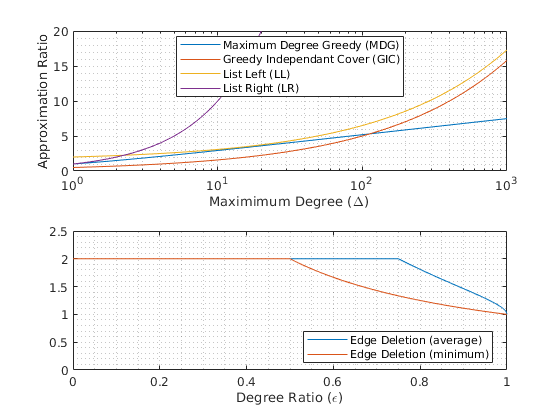
\includegraphics[width=0.8\linewidth]{ApproxRatioComp.png}
	\caption{Comparison of approximation ratios between several Vertex Cover heuristics}
	\Description{Comparison of approximation ratios between several Vertex Cover heuristics}
	\label{fig:approx_comp}
\end{figure}



The time complexity of the GIC algorithm as implemented is $O(n^2)$ where n is the number of nodes. As each node is selected via the minimum cardinality, at worst it has zero neighbors, so there would be at worst $n$ node selections. However in this case there would be 0 edge updates. For every neighbor that is present there are edge updates equal to the neighbors' cardinality. This can be at most $n-i$, where $i$ is the number of previous node selections. The complete complexity is then $O(\frac{n}{2}(n+1))$.

\subsection{Local Search 1 (specific descriptor)}

\subsubsection{Description}

The first local search algorithm we implement is simulated annealing. The main task is to find an appropriate cost evaluation function, and a definition of neighbor. 

For the first question, we define the cost as $$|V'|+\alpha\; \texttt{number of edges uncovered}$$ 
In the equation, $\alpha$ is a factor to define how important it is to cover all the edges while exploring new solutions. Then the main procedure is to start with an initial solution with a greedy algorithm and a large temperature, lower it gradually in each loop, find a neighbor and evaluate it, choose to switch to it or not using the probability given the evaluated cost change.

For the second question, we define neighbor in this algorithm as a set of vertices that differ from the current set with exactly one vertex, that is, the neighbor either has one more vertex in the set, or has all but one vertex compared with the current one. Using this definition, we can possibly go to the optimal solution in the sense that it is connected to the initial solution via the neighbor relationship.


\subsubsection{Pseudo Code}

\begin{algorithm}[H]
	\caption{Simulated Annealing}
	\SetAlgoLined
	\KwData{V,E}
	$init\_sol$ = init(V, E, neighbors)\;
	$best$ = (len($init\_sol$), $init\_sol$)\;
	$v\_set = init\_sol$\;
	$edges$ = edges covered by $v\_set$\;
	T = $T_{max}$\;
	\While{T $> 0$}
	{
		$next$ = random\_of($\{1,2,\dots,|V|\}$)\;
		$gain$ = 0\;
		\If{$next \in v\_set$}
		{
			$gain += 1$\;
			\For{$j \in neighbors[next]$}
			{
				\If{$j\notin v\_set$}{$gain -= \alpha$}
			}
		}
		\Else
		{
			$gain -= 1$\;
			\For{$j \in neighbors[next]$}
			{
				\If{$j\notin v\_set$}{$gain += \alpha$}
			}
		}
		$p = \min\{1, e^{\frac{gain}{T}}\}$\;
		\If{random(0,1) < $p$}
		{
			\If{$next \in v\_set$}
			{
				$v\_set$.remove($next$)\;
				\For{$j \in neighbors[next]$}
				{
					\If{$j\notin v\_set$}{edges.remove($next, j$)}\;
				}
			}
			\Else
			{
				$v\_set$.add($next$)\;
				\For{$j \in neighbors[next]$}
				{
					\If{$j\notin v\_set$}{edges.add($next, j$)}
				}
			}
		}
		\If{len($edges$) == $|E|$ \textbf{and} len($v\_set$)<$best[0]$}{$best = (len(v\_set), v\_set)$}
		$T -= T_{MAX}/k$\;
	}
	return ($best$)
\end{algorithm}

\subsubsection{Algorithm Analysis}

The pseudocode in last section shows how one whole loop of simulated annealing works, after each loop, if there's still more time available, the program simply start a new loop to try finding a better solution. Now let's analyze its time complexity of one complete loop. For a specific temperature, the main cost is for a randomly chosen vertex $next$, visiting all of its neighbors, which takes $O(|neighbors[next]|)$ time; then if the gain is positive or neighbor gets lucky, we update current vertex set and edge set, for which the main cost is also to visit all neighbors of $next$. Since this takes $k$ iterations, if we assume all vertices are visited almost evenly in long term, then on average the time complexity is $O(k|E|/|V| + |V| + |E|)$, where $|V|+|E|$ comes from the greedy algorithm to get the initial solution. As for space complexity, the main cost is to store the whole graph and the current vertex and edge set, which in total takes $O(|V|+|E|)$ space.\\\\

Overall, the strength of this local search algorithm is time efficiency, since each complete loop only takes $O(k|E|/|V| + |V| + |E|)$ time; moreover, as said before, because it is possible to visit any neighbor, and the initial solution is connected to an optimal solution under the neighbor relationship, it is guaranteed possible to reach the optimal solution. On the other hand, because this algorithm takes many hyper parameters $T_{MAX}$, $k$, $\alpha$, it is hard to find a good setting of them, especially when it encounters another input graph.

\subsection{Local Search 2 (specific descriptor)}

\subsubsection{Description}

\lipsum[1]

\subsubsection{Pseudo Code}

\begin{algorithm}[H]
	\caption{merge}
	\SetAlgoLined
	\KwData{B,C}
	$n_a$ = 0\;
	i = len(B)\;
	j = len(C)\;
	A = [0]*(i+j-2)\;
	\For{l = i+j-2; l $\geq$ 0; l-=1}{
		\uIf{i == 0}{
			A[0:l] = C[0:j]\;
			return (A,$n_a$)
		}
		\uElseIf{j == 0}{
			A[0:l] = B[0:i]\;
			return (A,$n_a$)
		}
		
		\uIf{C[j-1] $\geq$ B[i-1] }{
			A[l] = C[j-1]\;
			j = j-1\;
		}
		\uElse{
			A[l] = B[i-1]\;
			$n_a$ = $n_a$ + j\;
			i = i-1\;
		}
	}
	return (A,$n_a$)
\end{algorithm}

\subsubsection{Algorithm Analysis}

\lipsum[1]

\section{Empirical Evaluation}

a detailed description of your platform (CPU, RAM, language, compiler, etc.),
experimental procedure, evaluation criteria and obtained results (plots, tables, etc.). What is the
lower bound on the optimal solution quality that you can drive from the results of your approximation
algorithm and how far is it from the true optimum? How about from your branch-and-bound?

\begin{table}[H]
	\caption{Algorithm Performance}
	\label{tab:freq}
	\begin{tabular}{|l|c|c|c|c|c|c|c|c|c|c|c|c|c|}
		\toprule
		&\multicolumn{3}{c|}{Branch and Bound}&\multicolumn{3}{c|}{Construction Heuristic}&\multicolumn{3}{c|}{Local Search 1(avg of 10 runs)}&\multicolumn{3}{c|}{Local Search 2}\\
		\midrule
		Dataset&Time(s)&VC Value&RelErr&Time(s)&VC Value&RelErr&Time(s)&VC Value&RelErr&Time(s)&VC Value&RelErr&\\
		\midrule
		jazz&&&&0.0037&159&0.063&2.82&158.1&0.00063&&&\\
		karate&&&&0.0005&14&0.00&0.0.015&14.0&0.00&&&\\
		football&&&&0.0014&95&0.011&0.48&94.0&0.00&&&\\
		as-22july06&&&&0.21&3303&0.00&7.12&16729.1&4.06&&&\\
		hep-th&&&&0.098&3943&0.0043&4.98&5665.9&0.44&&&\\
		star&&&&0.24&7069&0.024&6.27&10440.8&0.51&&&\\
		star2&&&&0.21&4674&0.029&5.14&12055.4&1.65&&&\\
		netscience&&&&0.017&901&0.0022&4.68&986.3&0.097&&&\\
		email&&&&0.015&604&0.017&4.04&687.3&0.15&&&\\
		delaunay n10&&&&0.012&733&0.043&5.17&768.3&0.092&&&\\
		power&&&&0.051&2226&0.010&5.91&3108.2&0.41&&&\\
		\bottomrule
	\end{tabular}
\label{table:alg_perf}
\end{table}


\begin{figure}[p]
	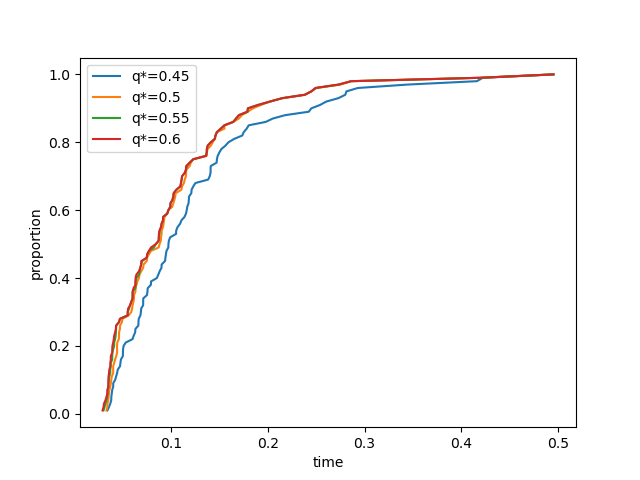
\includegraphics[width=\linewidth]{power_QRTD_LS1.png}
	\caption{QRTD of Power, Local Search 1}
\end{figure}


\begin{figure}[p]
	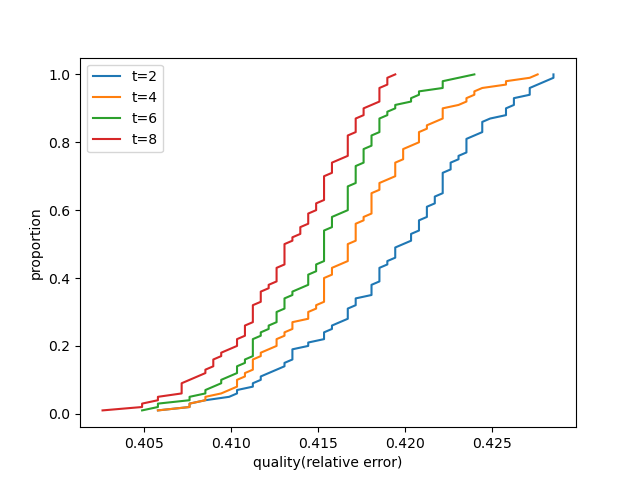
\includegraphics[width=\linewidth]{power_SQD_LS1.png}
	\caption{SQD of Power, Local Search 1}
\end{figure}

\begin{figure}[p]
	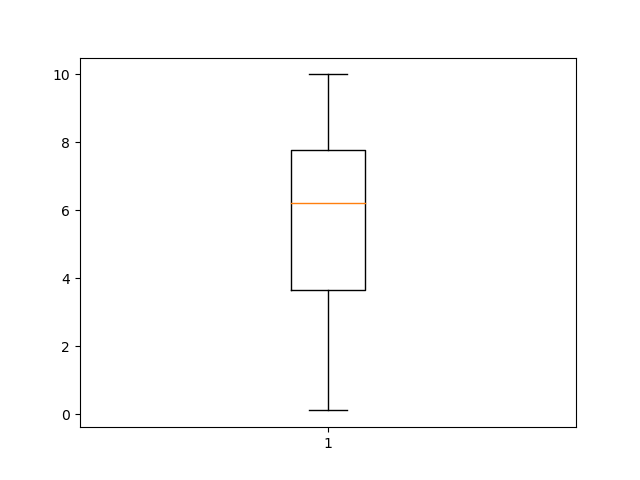
\includegraphics[width=\linewidth]{power_boxplot_LS1.png}
	\caption{boxplot of Power, Local Search 1}
\end{figure}


\begin{figure}[p]
	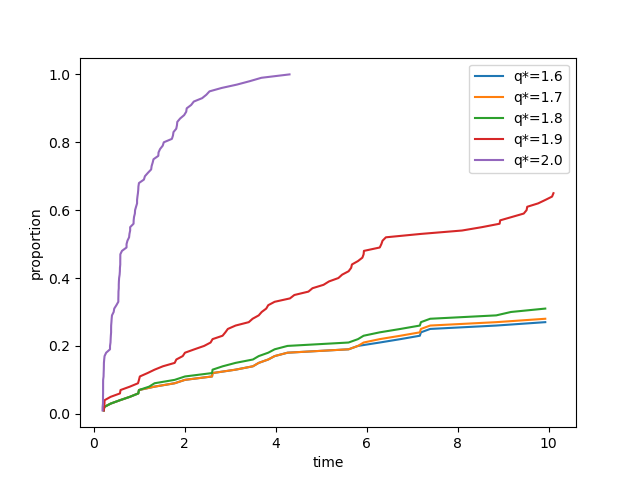
\includegraphics[width=\linewidth]{star2_QRTD_LS1.png}
	\caption{QRTD of Star2, Local Search 1}
\end{figure}


\begin{figure}[p]
	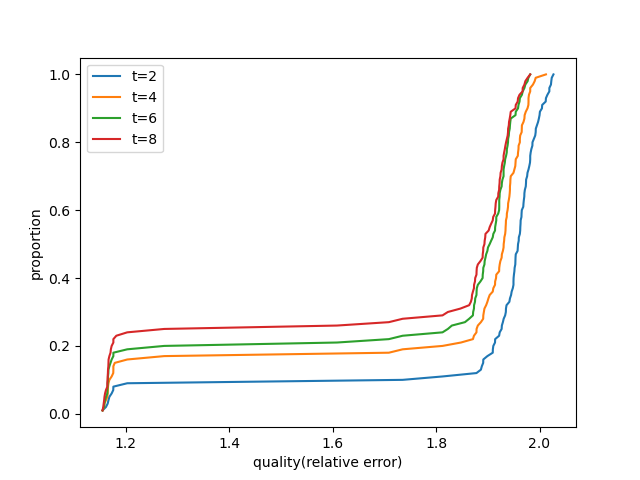
\includegraphics[width=\linewidth]{star2_SQD_LS1.png}
	\caption{SQD of Star2, Local Search 1}
\end{figure}

\begin{figure}[p]
	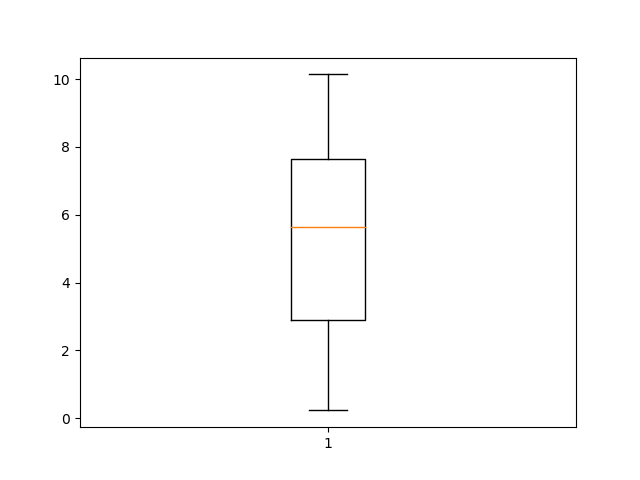
\includegraphics[width=\linewidth]{star2_boxplot_LS1.png}
	\caption{boxplot of Star2, Local Search 1}
\end{figure}



\section{Discussion}

a comparative analysis of how different algorithms perform with respect to your evaluation
criteria, or expected time complexity, etc


\section{Conclusion}



\section{Math Equations}
You may want to display math equations in three distinct styles:
inline, numbered or non-numbered display.  Each of the three are
discussed in the next sections.

\subsection{Inline (In-text) Equations}
A formula that appears in the running text is called an inline or
in-text formula.  It is produced by the \textbf{math} environment,
which can be invoked with the usual
\texttt{{\char'134}begin\,\ldots{\char'134}end} construction or with
the short form \texttt{\$\,\ldots\$}. You can use any of the symbols
and structures, from $\alpha$ to $\omega$, available in
\LaTeX~\cite{Lamport:LaTeX}; this section will simply show a few
examples of in-text equations in context. Notice how this equation:
\begin{math}
  \lim_{n\rightarrow \infty}x=0
\end{math},
set here in in-line math style, looks slightly different when
set in display style.  (See next section).

\subsection{Display Equations}
A numbered display equation---one set off by vertical space from the
text and centered horizontally---is produced by the \textbf{equation}
environment. An unnumbered display equation is produced by the
\textbf{displaymath} environment.

Again, in either environment, you can use any of the symbols and
structures available in \LaTeX\@; this section will just give a couple
of examples of display equations in context.  First, consider the
equation, shown as an inline equation above:
\begin{equation}
  \lim_{n\rightarrow \infty}x=0
\end{equation}
Notice how it is formatted somewhat differently in
the \textbf{displaymath}
environment.  Now, we'll enter an unnumbered equation:
\begin{displaymath}
  \sum_{i=0}^{\infty} x + 1
\end{displaymath}
and follow it with another numbered equation:
\begin{equation}
  \sum_{i=0}^{\infty}x_i=\int_{0}^{\pi+2} f
\end{equation}
just to demonstrate \LaTeX's able handling of numbering.

\section{Figures}

The ``\verb|figure|'' environment should be used for figures. One or
more images can be placed within a figure. If your figure contains
third-party material, you must clearly identify it as such, as shown
in the example below.
\begin{figure}[h]
  \centering
  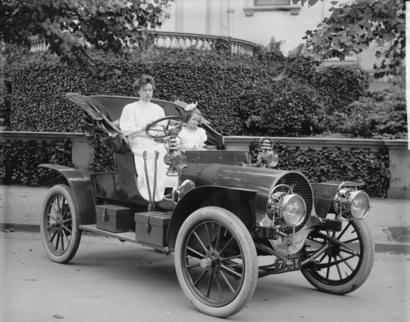
\includegraphics[width=\linewidth]{sample-franklin}
  \caption{1907 Franklin Model D roadster. Photograph by Harris \&
    Ewing, Inc. [Public domain], via Wikimedia
    Commons. (\url{https://goo.gl/VLCRBB}).}
  \Description{A woman and a girl in white dresses sit in an open car.}
\end{figure}

Your figures should contain a caption which describes the figure to
the reader.

Figure captions are placed {\itshape below} the figure.

Every figure should also have a figure description unless it is purely
decorative. These descriptions convey what’s in the image to someone
who cannot see it. They are also used by search engine crawlers for
indexing images, and when images cannot be loaded.

A figure description must be unformatted plain text less than 2000
characters long (including spaces).  {\bfseries Figure descriptions
  should not repeat the figure caption – their purpose is to capture
  important information that is not already provided in the caption or
  the main text of the paper.} For figures that convey important and
complex new information, a short text description may not be
adequate. More complex alternative descriptions can be placed in an
appendix and referenced in a short figure description. For example,
provide a data table capturing the information in a bar chart, or a
structured list representing a graph.  For additional information
regarding how best to write figure descriptions and why doing this is
so important, please see
\url{https://www.acm.org/publications/taps/describing-figures/}.

\section{Citations and Bibliographies}

The use of \BibTeX\ for the preparation and formatting of one's
references is strongly recommended. Authors' names should be complete
--- use full first names (``Donald E. Knuth'') not initials
(``D. E. Knuth'') --- and the salient identifying features of a
reference should be included: title, year, volume, number, pages,
article DOI, etc.

The bibliography is included in your source document with these two
commands, placed just before the \verb|\end{document}| command:
\begin{verbatim}
  \bibliographystyle{ACM-Reference-Format}
  \bibliography{bibfile}
\end{verbatim}
where ``\verb|bibfile|'' is the name, without the ``\verb|.bib|''
suffix, of the \BibTeX\ file.

Citations and references are numbered by default. A small number of
ACM publications have citations and references formatted in the
``author year'' style; for these exceptions, please include this
command in the {\bfseries preamble} (before the command
``\verb|\begin{document}|'') of your \LaTeX\ source:
\begin{verbatim}
  \citestyle{acmauthoryear}
\end{verbatim}


  Some examples.  A paginated journal article \cite{Fran10} \cite{Avis06} \cite{Hall97}

\section{Acknowledgments}

Identification of funding sources and other support, and thanks to
individuals and groups that assisted in the research and the
preparation of the work should be included in an acknowledgment
section, which is placed just before the reference section in your
document.

This section has a special environment:
\begin{verbatim}
  \begin{acks}
  ...
  \end{acks}
\end{verbatim}
so that the information contained therein can be more easily collected
during the article metadata extraction phase, and to ensure
consistency in the spelling of the section heading.

Authors should not prepare this section as a numbered or unnumbered {\verb|\section|}; please use the ``{\verb|acks|}'' environment.


%%
%% The acknowledgments section is defined using the "acks" environment
%% (and NOT an unnumbered section). This ensures the proper
%% identification of the section in the article metadata, and the
%% consistent spelling of the heading.
\begin{acks}
To Robert, for the bagels and explaining CMYK and color spaces.
\end{acks}

%%
%% The next two lines define the bibliography style to be used, and
%% the bibliography file.
\bibliographystyle{ACM-Reference-Format}
\bibliography{sample-base.bib}


\end{document}
\endinput
%%
%% End of file `sample-acmlarge.tex'.
